%%% The main file. It contains definitions of basic parameters and includes all other parts.

% Meta-data of your thesis (please edit)
\input metadata.tex

% Generate metadata in XMP format for use by the pdfx package
\input xmp.tex

%% Settings for single-side (simplex) printing
% Margins: left 40mm, right 25mm, top and bottom 25mm
% (but beware, LaTeX adds 1in implicitly)
\documentclass[12pt,a4paper]{report}
\setlength\textwidth{145mm}
\setlength\textheight{247mm}
\setlength\oddsidemargin{15mm}
\setlength\evensidemargin{15mm}
\setlength\topmargin{0mm}
\setlength\headsep{0mm}
\setlength\headheight{0mm}
% \openright makes the following text appear on a right-hand page
\let\openright=\clearpage

%% Settings for two-sided (duplex) printing
% \documentclass[12pt,a4paper,twoside,openright]{report}
% \setlength\textwidth{145mm}
% \setlength\textheight{247mm}
% \setlength\oddsidemargin{14.2mm}
% \setlength\evensidemargin{0mm}
% \setlength\topmargin{0mm}
% \setlength\headsep{0mm}
% \setlength\headheight{0mm}
% \let\openright=\cleardoublepage

%% If the thesis has no printed version, symmetric margins look better
% \documentclass[12pt,a4paper]{report}
% \setlength\textwidth{145mm}
% \setlength\textheight{247mm}
% \setlength\oddsidemargin{10mm}
% \setlength\evensidemargin{10mm}
% \setlength\topmargin{0mm}
% \setlength\headsep{0mm}
% \setlength\headheight{0mm}
% \let\openright=\clearpage

%% Generate PDF/A-2u
\usepackage[a-2u]{pdfx}

%% Prefer Latin Modern fonts
\usepackage{lmodern}
% If we are not using LuaTeX, we need to set up character encoding:
\usepackage{iftex}
\ifpdftex
\usepackage[utf8]{inputenc}
\usepackage[T1]{fontenc}
\usepackage{textcomp}
\fi

%% Further useful packages (included in most LaTeX distributions)
\usepackage{amsmath}        % extensions for typesetting of math
\usepackage{amsfonts}       % math fonts
\usepackage{amsthm}         % theorems, definitions, etc.
\usepackage{bm}             % boldface symbols (\bm)
\usepackage{booktabs}       % improved horizontal lines in tables
\usepackage{caption}        % custom captions of floating objects
\usepackage{dcolumn}        % improved alignment of table columns
\usepackage{floatrow}       % custom float environments
\usepackage{graphicx}       % embedding of pictures
\usepackage{indentfirst}    % indent the first paragraph of a chapter
\usepackage[nopatch=item]{microtype}   % micro-typographic refinement
\usepackage{paralist}       % improved enumerate and itemize
\usepackage[nottoc]{tocbibind} % makes sure that bibliography and the lists
			    % of figures/tables are included in the table
			    % of contents
\usepackage{xcolor}         % typesetting in color

% The hyperref package for clickable links in PDF and also for storing
% metadata to PDF (including the table of contents).
% Most settings are pre-set by the pdfx package.
\hypersetup{unicode}
\hypersetup{breaklinks=true}

% Packages for computer science theses
\usepackage{algpseudocode}  % part of algorithmicx package
\usepackage{algorithm}
\usepackage{fancyvrb}       % improved verbatim environment
\usepackage{listings}       % pretty-printer of source code

% You might want to use cleveref for references
% \usepackage{cleveref}

% Set up formatting of bibliography (references to literature)
% Details can be adjusted in macros.tex.
%
% BEWARE: Different fields of research and different university departments
% have their own customs regarding bibliography. Consult the bibliography
% format with your supervisor.
%
% The basic format according to the ISO 690 standard with numbered references
\usepackage[natbib,style=iso-numeric,sorting=none]{biblatex}
% ISO 690 with alphanumeric references (abbreviations of authors' names)
%\usepackage[natbib,style=iso-alphabetic]{biblatex}
% ISO 690 with references Author (year)
%\usepackage[natbib,style=iso-authoryear]{biblatex}
%
% Some fields of research prefer a simple format with numbered references
% (sorting=none tells that bibliography should be listed in citation order)
%\usepackage[natbib,style=numeric,sorting=none]{biblatex}
% Numbered references, but [1,2,3,4,5] is compressed to [1-5]
%\usepackage[natbib,style=numeric-comp,sorting=none]{biblatex}
% A simple format with alphanumeric references:
%\usepackage[natbib,style=alphabetic]{biblatex}

% Load the file with bibliography entries
\addbibresource{bibliography.bib}

% Our definitions of macros (see description inside)
\input macros.tex

%%% Title page and various mandatory informational pages
\begin{document}
%%% Title page of the thesis and other mandatory pages

%%% Inscriptions at the opening page of the hard cover

% We usually do not typeset the hard cover, but if you want to do it, change \iffalse to \iftrue
\iffalse

\pagestyle{empty}
\hypersetup{pageanchor=false}
\begin{center}

\large
Charles University

\medskip

Faculty of Mathematics and Physics

\vfill

{\huge\bf\ThesisTypeTitle}

\vfill

{\huge\bf\ThesisTitle\par}

\vfill
\vfill

\hbox to \hsize{\YearSubmitted\hfil \ThesisAuthor}

\end{center}

\newpage\openright
\setcounter{page}{1}

\fi

%%% Title page of the thesis

\pagestyle{empty}
\hypersetup{pageanchor=false}
\begin{center}

\centerline{\mbox{\includegraphics[width=166mm]{img/logo-en.pdf}}}

\vspace{-8mm}
\vfill

{\bf\Large\ThesisTypeTitle}

\vfill

{\LARGE\ThesisAuthor}

\vspace{15mm}

{\LARGE\bfseries\ThesisTitle\par}

\vfill

\Department

\vfill

{
\centerline{\vbox{\halign{\hbox to 0.45\hsize{\hfil #}&\hskip 0.5em\parbox[t]{0.45\hsize}{\raggedright #}\cr
Supervisor of the \ThesisTypeName{} thesis:&\Supervisor \cr
\ifx\ThesisType\TypeRig\else
\noalign{\vspace{2mm}}
Study programme:&\StudyProgramme \cr
\fi
}}}}

\vfill

Prague \YearSubmitted

\end{center}

\newpage

%%% A page with a solemn declaration to the thesis

\openright
\hypersetup{pageanchor=true}
\vglue 0pt plus 1fill

\noindent
I declare that I carried out this \ThesisTypeName{} thesis on my own, and only with the cited
sources, literature and other professional sources.
I understand that my work relates to the rights and obligations under the Act No.~121/2000 Sb.,
the Copyright Act, as amended, in particular the fact that the Charles
University has the right to conclude a license agreement on the use of this
work as a school work pursuant to Section 60 subsection 1 of the Copyright~Act.

\vspace{10mm}

\hbox{\hbox to 0.5\hsize{%
In \hbox to 6em{\dotfill} date \hbox to 6em{\dotfill}
\hss}\hbox to 0.5\hsize{\dotfill\quad}}
\smallskip
\hbox{\hbox to 0.5\hsize{}\hbox to 0.5\hsize{\hfil Author's signature\hfil}}

\vspace{20mm}
\newpage

%%% Dedication

\openright

\noindent
\Dedication

\newpage

%%% Mandatory information page of the thesis

\openright
{\InfoPageFont

\vtop to 0.5\vsize{
\setlength\parindent{0mm}
\setlength\parskip{5mm}

Title:
\ThesisTitle

Author:
\ThesisAuthor

\DeptType:
\Department

Supervisor:
\Supervisor, \SupervisorsDepartment

Abstract:
\Abstract

Keywords:
{\def\sep{\unskip, }\ThesisKeywords}

\vfil
}

% In Czech study programmes, it is mandatory to include Czech meta-data:

\ifx\StudyLanguage\LangCS

\vtop to 0.49\vsize{
\setlength\parindent{0mm}
\setlength\parskip{5mm}

Název práce:
\ThesisTitleCS

Autor:
\ThesisAuthor

\DeptTypeCS:
\DepartmentCS

Vedoucí bakalářské práce:
\Supervisor, \SupervisorsDepartmentCS

Abstrakt:
\AbstractCS

Klíčová slova:
{\def\sep{\unskip, }\ThesisKeywordsCS}

\vfil
}

\fi

}

\newpage

%%% Further pages will be numbered
\pagestyle{plain}


%%% A page with automatically generated table of contents of the thesis

\tableofcontents

%%% Each chapter is kept in a separate file
\chapter*{Introduction}
\addcontentsline{toc}{chapter}{Introduction}

In recent years, mobile technologies have advanced rapidly, which had a significant impact on various aspects of our lives, especially in education and culture. Museums, for example, are now introducing mobile technologies to increase visitor engagement and learning experiences. Traditional museum tours are often based on static information stands and guided tours, which may not match the pace and preferences of individual visitors. To solve this problem, we propose a mobile application that uses real-time image classification to create an interactive and personalized museum guide.

The core of this application is a fine-tuned MobileNet neural network converted to TensorFlow Lite for efficient image classification on mobile devices. The model has been trained on a dataset with frames extracted from videos of museum exhibits. 

Users of the application need to point the camera of their mobile device at the exhibit. The app will automatically take pictures at regular intervals and classify them into one of several predefined categories. After successful classification, the application extracts detailed information about the exhibit from a local database and displays it to the user. This process turns a museum visit into an interactive process where information is easily accessible.

The development of this application included several key steps: video recording and frame extraction, model training and fine-tuning, Android application development and model integration into this application. Each stage presented unique tasks and required special technical solutions, which are discussed in detail in this paper.

The main goal of this project is to demonstrate how mobile image classification can improve the experience of museum visitors. By automating the process of information recognition and retrieval, the application reduces the need for physical guides and static information boards, allowing visitors to explore exhibits at their own pace and according to their interests.

In conclusion, this work aims to provide a comprehensive report on the development and implementation of a mobile application for real-time image classification of museum exhibits. It highlights the technical and practical aspects, as well as the potential benefits for museums and their visitors. Through this work, we hope to contribute to the ongoing efforts to integrate technology into the cultural and educational context, making learning more accessible and fun.
\chapter{Related Work}

With the advent of mobile technology, museums are exploring new ways to increase visitor engagement in the learning process. Mobile applications and interactive guides are being used to conduct personalized tours, receive information in augmented reality, and more.

\section*{Mobile Applications in Museums}

Several projects have demonstrated the potential of mobile applications to improve the museum experience. For example, the development of mobile applications such as the ``Louvre Visit, Tours \& Guide`` \cite{louvre_app} and the ``British Museum Audio`` \cite{british_museum_app} has shown that visitors can benefit from access to a digital guidebook that not only provides additional information about the exhibits, but also shares practical information, navigation, and flexible self-guided tours.

However, to access information, these applications mainly use manual user input, such as scanning QR codes or entering exhibit numbers. Despite its effectiveness, this approach lacks the speed and seamlessness that can be achieved with more advanced technologies such as image recognition and real-time classification.

\section*{Image Classification in Cultural Heritage Institutions}

The integration of image recognition technology into museum applications represents a significant step forward in creating a more interactive and responsive user experience. For example, a project called ``CHESS`` (Cultural Heritage Experiences through Socio-personal interactions and Storytelling) \cite{chess_project}, co-funded by the European Commission, has explored the use of image recognition to identify works of art and provide augmented reality experience. Such systems allow visitors to point their devices at the exhibits to instantly receive detailed information, thereby improving the learning process by minimizing the effort required to interact with the content.

\section*{Summary}

In summary, the integration of mobile applications and image recognition models into the museum experience has demonstrated great potential in increasing visitor engagement and learning. While traditional mobile guides provide valuable information, the addition of real-time image classification represents a significant step forward in providing seamless interaction. As museums continue to introduce these technologies, visitors' experiences are likely to become more personalized, dynamic, and informative.
\chapter{Theoretical Background}

\section{Convolutional Neural Networks (CNNs)}

\subsection{Introduction to CNNs}

Convolutional Neural Networks (CNNs) are a class of deep learning models that have gained widespread popularity due to their ability to effectively analyze visual data. Originally inspired by the organization of the animal visual cortex, CNNs are a perfect tool for image recognition tasks.

A distinctive feature of CNNs is their ability to capture local dependencies in images using convolutional layers. These layers apply trainable filters (or kernels) over the input image to detect various features such as edges, textures, and patterns. As the network deepens, it gradually captures more complex and abstract features, which allows for highly accurate image classification.

\subsection{Architecture of CNNs}

A typical CNN architecture consists of several key components: an input layer, convolutional layers, pooling layers, and fully connected layers. Each component plays a specific role in processing the input data and contributing to the overall functionality of the network.

\begin{figure}[h]
    \centering
    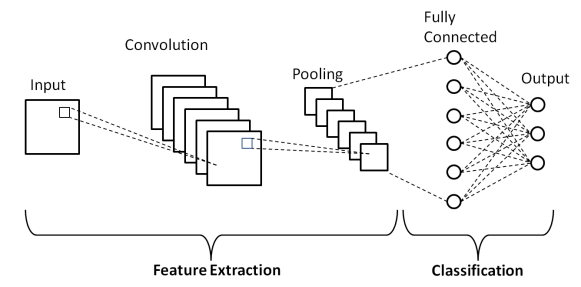
\includegraphics[width=0.7\textwidth]{img/cnn-architecture.png}
    \caption{Illustration of a CNN architecture. Source: \href{https://www.researchgate.net/publication/336805909_A_High-Accuracy_Model_Average_Ensemble_of_Convolutional_Neural_Networks_for_Classification_of_Cloud_Image_Patches_on_Small_Datasets}{ResearchGate article.}}
    \label{fig:cnn-architecture}
\end{figure}

\subsubsection{Convolutional Layers}

Convolutional layers are the main building block of a CNN architecture. They apply a set of filters over the input image, where each filter slides (or convolves) across the image to produce a feature map. This operation helps the network learn spatial hierarchies of features, where earlier layers might detect simple edges or textures, and deeper layers capture more complex structures like shapes or even entire objects.

The mathematical operation behind convolution involves multiplying each filter's weights by the corresponding pixel values in the input image and summing the results. This process is repeated as the filter moves across the image, resulting in a feature map that highlights the presence of the feature detected by the filter.

Mathematically, the convolution operation for a single filter can be expressed as:

\[
\text{FeatureMap}(i,j) = \sum_{m,n} I_{i-m,j-n} W_{m,n} + b
\]

where \(W\) represents the filter weights, \(I\) represents the input image pixel values, and \(b\) is the bias term.

\subsubsection{Activation Functions}

After convolution, the output feature map is passed through a non-linear activation function, typically the Rectified Linear Unit (ReLU). The ReLU activation function is defined as:

\[
ReLU(x) = \max(0, x)
\]

ReLU introduces non-linearity into the model, which is needed in order to learn more complex patterns in the data. Other activation functions, for example hyperbolic tangent (tanh), can also be used, but ReLU is preferred in most CNN architectures due to its simplicity and effectiveness in avoiding the vanishing gradient problem.

\subsubsection{Pooling Layers}

Pooling layers, often placed between consecutive convolutional layers, are used to reduce the dimensions of the feature maps. This operation reduces the network's computational complexity and makes the learned features more invariant to small translations of the input image.

The most common pooling operation is max pooling, which selects the maximum value from each region of the feature map. The formula for max pooling over a 2x2 region is:

\[
\text{MaxPool}(i,j) = \max \{ I_{2i,2j}, I_{2i,2j+1}, I_{2i+1,2j}, I_{2i+1,2j+1} \}
\]

Another popular type of pooling operation is average pooling, which computes the region's average value instead of the maximum.

Overall, pooling layers gradually reduce the spatial size of the image representation, making the network more efficient while retaining the most important features. 

\subsubsection{Fully Connected Layers}

After several convolutional and pooling layers, the resulting feature maps are flattened into a one-dimensional vector to be processed by one or more fully connected layers. These layers function like a standard neural network, where each neuron is linked to every neuron in the next layer. Finally, the last fully connected layer, called the output layer, performs the final classification.

The CNN's output layer typically uses a softmax activation function for multi-class classification tasks. The softmax function converts the output scores into probabilities, allowing the network to assign a class label to the input image.

\subsection{Conclusion}

CNNs have been successfully used to solve various image classification tasks, including object detection, face recognition, and medical image analysis. In the context of museum applications, CNNs are used to classify and recognize various types of exhibits, ranging from paintings and sculptures to historical artifacts. By fine-tuning pre-trained CNN models on museum-specific datasets, it is possible to achieve high accuracy in identifying exhibits, thereby enhancing the visitor experience.

\section{MobileNet}

MobileNet is a class of efficient convolutional neural networks specifically designed for mobile and embedded vision applications. Introduced by Howard et al. \cite{howard_mobilenet}, MobileNet addresses the need for high-performance neural networks that can work efficiently on devices with limited resources (e.g., smartphones).

\subsection{Architecture of MobileNet}

The core innovation of MobileNet is the use of depthwise separable convolutions, which break down the standard convolution operation into two simpler steps: depthwise convolution (applying a single filter per input channel) and pointwise convolution (combining the output channels). This approach significantly reduces the number of calculations (23x fewer multiplications for an 8x8x3 image) and model size, making MobileNet fast and lightweight.

\begin{figure}[h]
    \centering
    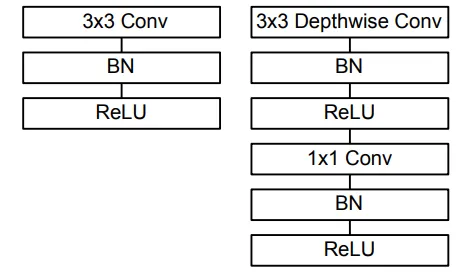
\includegraphics[width=0.7\textwidth]{img/mobilenet.png}
    \caption{Left: Standard Convolutional layer, Right: Depthwise Separable Convolutional layers in MobileNet. Source: image from the original paper.}
    \label{fig:mobilenet}
\end{figure}

\subsection{MobileNet Versions}

There are three versions of the MobileNet architecture, each improving upon the last in terms of efficiency and accuracy:

\textbf{MobileNetV1} was the first iteration, known for being ten times faster and smaller than the VGG16 architecture, making it a popular choice for mobile applications due to its significant reduction in computational resources \cite{pandrii_mobilenet}.

\textbf{MobileNetV2} introduced inverted residual blocks with linear bottlenecks, which enhanced the model's ability to learn more efficient representations. This version is approximately 30\% smaller and 0.3 times faster than MobileNetV1 while being 1\% more accurate \cite{pandrii_mobilenet}.

\textbf{MobileNetV3} builds upon the improvements of V2 by incorporating advances such as Neural Architecture Search (NAS) and Squeeze-and-Excitation (SE) modules. MobileNetV3 is twice as fast and 30\% smaller than V2 but with a slight trade-off in accuracy, being 3\% less accurate than MobileNetV2 \cite{pandrii_mobilenet}.

\textbf{Note on Model Choice:} Despite the improvements in MobileNetV3, MobileNetV2 was chosen for this thesis due to its optimal balance between accuracy and efficiency. While V3 offers better speed and smaller size, the slight reduction in accuracy was not suitable for the high accuracy requirements of this project.

\subsection{Conclusion}

Thanks to its efficient design, MobileNet offers a well-balanced architecture ideal for real-time applications on mobile devices. In this thesis, MobileNet's lightweight structure is crucial for effectively and accurately classifying museum exhibits, providing visitors with enhanced learning experiences while maintaining optimal performance on mobile hardware.

\section{Transfer Learning}

\subsection{Introduction to Transfer Learning}

Transfer learning is a machine learning technique of using knowledge gained during the execution of one task to improve the performance of another related task. Instead of building and training a new model from scratch, scientists and engineers can use pre-trained models as a starting point, reducing the need for large amounts of data and computational resources.

In traditional machine learning, models are usually trained from scratch using a large dataset for a specific task. This process involves learning feature representations from the raw data, which can be time-consuming and computationally intensive. However, the early layers of neural networks often learn general features like edges and textures that are useful across tasks, so transfer learning takes advantage of these general features by reusing the early layers of a pre-trained model and fine-tuning the later layers on the target task. The most common approach to transfer learning involves:

1. \textbf{Pre-training:} A model is first trained on a large source dataset with extensive labeled examples (e.g., ImageNet). During this phase, the model learns to extract general features from the input data.

2. \textbf{Fine-tuning:} The pre-trained model is then adapted to the target task by continuing training on a smaller, task-specific dataset. This process fine-tunes the model's weights to better fit the characteristics of the target data while retaining the knowledge acquired during pre-training.

\subsection{Transfer Learning in CNNs}

Transfer learning is widely used in the context of CNNs, especially for image classification tasks. During transfer learning, the early layers of a pre-trained CNN are often frozen (i.e., their weights are kept constant), and only the deeper layers are fine-tuned. This approach keeps the general feature extraction capabilities of the early layers, which are often relevant across different tasks, while adapting the model to the specific characteristics of the target data.

\subsection{Transfer Learning in Museum Exhibit Classification}

In the context of museum exhibit classification, transfer learning is beneficial due to the limited availability of labeled data for training. Museum exhibits vary widely in style, material, and content, making it difficult to compile a comprehensive dataset. By using a pre-trained CNN model like MobileNet, which has been trained on a large, diverse dataset such as ImageNet, it is possible to effectively classify museum exhibits with a smaller, domain-specific dataset.

\subsection{Conclusion}

Transfer learning enables the reuse of pre-trained models to solve new tasks with limited data and resources. In this thesis, transfer learning is crucial for developing an efficient and accurate model for museum exhibit classification, ensuring high-quality performance on mobile devices.

\chapter*{Conclusion}
\addcontentsline{toc}{chapter}{Conclusion}

In this thesis, we explored, implemented, and evaluated a mobile application capable of recognizing museum exhibits in real time. The primary objective was to provide museum visitors with quick, accurate access to information about exhibits directly through their Android smartphones.

We began by preparing a suitable dataset by recording videos of exhibits and extracting individual frames. Care was taken to ensure balanced representation of each exhibit, extracting frames at regular intervals and subsequently labeling them using metadata stored in a CSV file. This approach allowed us to create a well-structured dataset for our task.

The initial exploration of potential approaches identified two main solutions for achieving accurate image recognition: the embedding-based similarity search and direct classification using transfer learning. The first method, embedding-based similarity search, although highly flexible, was soon discarded due to practical limitations, notably the high computational requirements and significant storage overhead of embeddings on mobile devices. Alternatively, direct classification through transfer learning proved to be the most suitable option, balancing accuracy, performance, ease of integration, and storage efficiency.

For the classification architecture, MobileNetV2 was chosen due to its compact and efficient design aimed at mobile environments. Through experimentation with different configurations --- such as batch sizes, number of layers, dropout rates, and fine-tuning --- we arrived at a final optimized model that achieved validation accuracy of approximately 95.9\%.

An analysis of misclassifications revealed that errors mostly occurred on visually similar exhibits or when multiple objects appeared within a single image. To mitigate this, the application's user interface includes not only the model's top prediction but also several alternative suggestions (in a non-intrusive manner). This allows users to easily access information about exhibits, even when predictions are not entirely accurate.

The developed Android application integrates TensorFlow Lite for lightweight on-device inference and employs CameraX for simple, efficient camera access. The application includes multiple screens --- from a home and gallery view to dedicated exhibit detail and real-time scanner screens --- organized clearly and intuitively. Additionally, a debug mode was implemented for convenient monitoring and adjusting classification thresholds and inference time evaluation.

Real-world testing was conducted at the Museum of Decorative Arts in Prague (UPM). Practical evaluation on a subset of 80 museum exhibits yielded an accuracy of around 93.75\%, closely matching expectations derived from validation results. Misclassifications again typically involved visually similar exhibits, yet the correct exhibit usually appeared within the offered alternative suggestions. Furthermore, inference was fast enough --- around 120--150 ms --- to provide smooth, responsive real-time interaction.

Nevertheless, there are several practical ways to build upon this work. Expanding the dataset is always beneficial, as training on more images under various conditions generally helps models achieve better generalization. Additionally, future work could explore alternative neural network architectures apart from MobileNetV2; examples include EfficientNet Lite or ShuffleNet, both specifically designed to run efficiently on mobile devices while maintaining good classification accuracy. It could also be beneficial to experiment with entirely different approaches, including object detection techniques such as YOLO or SSD. Object detection would enable simultaneous localization and recognition of multiple exhibits within a single camera frame, directly addressing one of the challenges identified during evaluation. Furthermore, hybrid approaches that combine CNN-based models with classical image descriptors or utilize additional sensor data (e.g., Bluetooth beacons or NFC tags) could offer increased robustness and improved recognition performance in challenging scenarios.

Overall, this work successfully demonstrated that modern machine learning methods in combination with optimized model architectures and mobile technologies can effectively support real-time museum exhibit recognition. The resulting application not only performed reliably within a controlled evaluation but also showed potential applicability to broader museum contexts. With incremental improvements and adaptations, such tools could meaningfully assist visitors, providing convenient, immediate, and easy-to-access information right at their fingertips.


%%% Bibliography
%%% Bibliography (literature used as a source)
%%%
%%% We employ biblatex to construct the bibliography. It processes
%%% citations in the text (e.g., the \cite{...} macro) and looks up
%%% relevant entries in the bibliography.bib file.
%%%
%%% See also biblatex settings in thesis.tex.

%%% Generate the bibliography. Beware that if you cited no works,
%%% the empty list will be omitted completely.

% We let bibliography items stick out of the right margin a little
\def\bibfont{\hfuzz=2pt}

\printbibliography[heading=bibintoc]

%%% If case you prefer to write the bibliography manually (without biblatex),
%%% you can use the following. Please follow the ISO 690 standard and
%%% citation conventions of your field of research.

% \begin{thebibliography}{99}
%
% \bibitem{lamport94}
%   {\sc Lamport,} Leslie.
%   \emph{\LaTeX: A Document Preparation System}.
%   2nd edition.
%   Massachusetts: Addison Wesley, 1994.
%   ISBN 0-201-52983-1.
%
% \end{thebibliography}


%%% Figures used in the thesis (consider if this is needed)
\listoffigures

%%% Tables used in the thesis (consider if this is needed)
%%% In mathematical theses, it could be better to move the list of tables to the beginning of the thesis.
\listoftables

%%% Abbreviations used in the thesis, if any, including their explanation
%%% In mathematical theses, it could be better to move the list of abbreviations to the beginning of the thesis.
\chapwithtoc{List of Abbreviations}

%%% Doctoral theses must contain a list of author's publications
\ifx\ThesisType\TypePhD
\chapwithtoc{List of Publications}
\fi

%%% Attachments to the thesis, if any. Each attachment must be referred to
%%% at least once from the text of the thesis. Attachments are numbered.
%%%
%%% The printed version should preferably contain attachments, which can be
%%% read (additional tables and charts, supplementary text, examples of
%%% program output, etc.). The electronic version is more suited for attachments
%%% which will likely be used in an electronic form rather than read (program
%%% source code, data files, interactive charts, etc.). Electronic attachments
%%% should be uploaded to SIS. Allowed file formats are specified in provision
%%% of the rector no. 72/2017. Exceptions can be approved by faculty's coordinator.
\appendix
\chapter{Attachments}

\section{First Attachment}

\end{document}
